\section{Appendix}

In this appendix, we present more formally the matching functions used as baselines for our study in (Section~\ref{sec:supp_matching}), as well as extra experiments that study the impact of different hyper-parameters and present results of different task setups (Section~\ref{sec:supp_ablations}). 


\begin{figure*}[t]
\centering 
\begin{tabular}{cc}
    \vspace{-5pt}  
    \begin{subfigure}{0.63\textwidth}
        \includegraphics[width=\textwidth]{figures/method/temporal_matching.pdf}
        \vspace{-15pt}
        \caption{}
        \label{fig:matching_learning}
    \end{subfigure}
    \begin{subfigure}{0.3\textwidth}
        \includegraphics[width=\textwidth]{figures/method/non_temporal_matching.pdf}
        \vspace{-15pt}
        \caption{}
        \label{fig:non_temporal_matching_learning}
    \end{subfigure}
\end{tabular}
    \vspace{-2ex}
    \caption{\textbf{Matching functions on the temporal similarity matrix $M$.} We show how each method estimates a scalar video-to-video similarity given the input pairwise similarity matrix. The functions can be classified as a) temporal or b) non-temporal whether they use the temporal position of the features or not.
    \label{fig:matching}
    \vspace{-3ex}
    }
\end{figure*}
\subsection{Baseline matching functions}
\label{sec:supp_matching}

In this section, we describe the different matching functions used as our study's baseline\alert{, and depicted in Figure~\ref{fig:matching}}.
Some matching functions use temporal information by leveraging the absolute or relative position of the pairwise similarities $m_{ij}$. The matching functions that use temporal information are called \emph{temporal} whereas the others are called \emph{non-temporal}.


\subsubsection{Temporal matching functions.}

We provide a list of the temporal matching functions implemented in this study as baselines. Some of them were already introduced in prior work.

\noindent
\myparagraph{Diagonal (Diag)} is used as a baseline in prior work \cite{otam}. It is given by $s(M)= \displaystyle \nicefrac{\sum_{ij} m_{ii}}{n}$. It assumes temporally aligned video pairs.

\noindent
\myparagraph{OTAM}~\cite{otam} uses and extends Dynamic Time Warping~\cite{Muller2007DTW} to find an alignment path on $M$ over which similarities are averaged to produce the video-to-video similarity. A differentiable variant is used for training.

\noindent
\myparagraph{Flatten+FC (Linear)} is a simple baseline we use to learn temporal matching by flattening $M$ and feeding it to a Fully Connected (FC) layer without bias and with a single scalar output. Video-to-video similarity is therefore given by $s(M) = \sum_{ij} w_{ij} m_{ij}$, where $w_{ij}$ are learnable parameters which are $n^2$ in total.

\noindent
\myparagraph{ViSiL}~\cite{visil} is an approach originally introduced for the task of video retrieval. We apply it to few-shot action recognition for the first time. A small Fully Convolutional Network (FCN) is applied on $M$. Its output is a filtered temporal similarity matrix, and the Chamfer similarity is applied on it. The filtering is performed according to the small temporal context captured by the small receptive field of this network.

\subsubsection{Non-temporal matching functions.} 
We provide a list of the non-temporal matching functions that were implemented in this study as baselines. 

\noindent
\myparagraph{Mean} is used as a baseline in prior work \cite{otam}. It is given by $s(M)= \displaystyle \nicefrac{\sum_{ij} m_{ij}}{n^2}$. It supposes all the clip pairs should contribute equally to the similarity score.

\noindent
\myparagraph{Max} is used as a baseline in prior work \cite{otam}. It is given by $s(M)= \max_{ij} m_{ij}$.
It supposes that selecting the best matching clip pair is enough to recognize the action. 




\subsection{Additional ablations and impact of hyper-parameters}
\label{sec:supp_ablations}
In this section, we present additional ablations to evaluate the impact of the feature projection head, the ordering of the tuples, and the number of examples per class used in the support set. We also report the impact of using the different variants for the \kinetics and \ucf datasets.


\begin{table}[t]
\caption{\textbf{Impact of learning a feature projection on performance of matching-based methods}. $^\dagger$ denotes hand-crafted matching methods, \ie no training is performed for the cases where a feature projection is not learned.
\label{tab:feature_embeddings_dataloader}
}
\vspace{1ex}
\centering
\vspace{2ex}

\setlength\extrarowheight{3pt}
    \resizebox{\linewidth}{!}{
    \setlength{\tabcolsep}{12pt}
    \begin{tabular}{ l c cc cc} 
    \toprule
         \multirow{2}{*}{Method}  & Learned       & \multicolumn{2}{c}{\ssvtwo} & \multicolumn{2}{c}{\kinetics}  \\
                                  & Proj.       &  \oneshot & \fiveshot & \oneshot & \fiveshot \\
         \midrule
         Max$^\dagger$ &    & 63.40 & 75.80 & 94.90 & 97.50  \\ 
         Max &  \checkmark & 64.97 & 78.97 &  95.27 & 98.30   \\
         & & \diffup{1.57} & \diffup{3.17} & \diffup{0.37} & \diffup{0.80} \\
          \midrule
         Chamfer++ (l=3)$^\dagger$ &    & 64.50 & 79.50 & 94.10 & 98.10  \\ 
         Chamfer++ (l=3) &  \checkmark  & 67.83 & 81.60 &  96.10 & 98.30   \\
         & & \diffup{3.33} & \diffup{2.10} & \diffup{2.00} & \diffup{0.20} \\
          \midrule
         Mean$^\dagger$ &    & 61.40 & 75.40 & 92.50 & 97.50  \\ 
         Mean &  \checkmark & 65.77 & 79.13 &  95.53 & 98.10   \\
         & & \diffup{4.37} & \diffup{3.73} & \diffup{3.03} & \diffup{0.60} \\
          \midrule
         OTAM~\cite{otam}$^\dagger$ &  & 63.70  & 76.40 & 93.70 & 97.90 \\ 
         OTAM~\cite{otam} & \checkmark & 67.10  & 80.23 & 95.93 & 98.37   \\ 
         & & \diffup{3.40} & \diffup{3.83} & \diffup{2.23} & \diffup{0.47} \\
    \bottomrule
    \end{tabular}
    }

\vspace{1ex}
\end{table}

\begin{table}[t]
\vspace{1ex}
\caption{\textbf{Impact of the dimension size of the feature projection head} for Chamfer++ using ordered-tuples and $l=3$.
\label{tab:feature_projection_dimension}
}
\centering

\vspace{2ex}

\resizebox{\linewidth}{!}
{
\small
\setlength\extrarowheight{-1pt}
\setlength{\tabcolsep}{12pt}
\begin{tabular}{ l c cc cc} 
\toprule
    \multirow{2}{*}{Method}  & $D$ &  \multicolumn{2}{c}{\ssvtwo} & \multicolumn{2}{c}{\kinetics}  \\
    & &  \oneshot & \fiveshot & \oneshot & \fiveshot  \\
     \midrule
     Chamfer++ (l=3)  &  & 64.5 \stddev{0.0}& 79.5 \stddev{0.0} & 94.1 \stddev{0.0}& 98.1 \stddev{0.0} \\
     Chamfer++ (l=3)  &  512 & 67.3 \stddev{0.2} & 81.2 \stddev{0.0} & 95.9 \stddev{0.1} &  98.2 \stddev{0.1}  \\
     Chamfer++ (l=3)  &  1024 & 67.8 \stddev{0.3} & 81.3  \stddev{0.1} & 96.1 \stddev{0.2} & 98.3 \stddev{0.0}  \\
     Chamfer++ (l=3)  &  1152 &  67.8 \stddev{0.2} & 81.6 \stddev{0.1} & 96.1 \stddev{0.1}& 98.3 \stddev{0.0}  \\
     Chamfer++ (l=3)  &  2048 & 67.9  \stddev{0.0} & 81.8 \stddev{0.2} & 96.1 \stddev{0.1} &  98.3 \stddev{0.0}  \\
\bottomrule
\end{tabular}
    }


\vspace{1ex}
\end{table}


\subsubsection{The impact of the projection layer} for matching methods is validated in Table~\ref{tab:feature_embeddings_dataloader}.
The performance is consistently improved on all setups and methods by including and learning a projection layer.
Although the backbone is trained with TSL on the same meta-train set, the projection layer allows features and values in the temporal similarity matrix to better align with each matching process.

\subsubsection{Projection head dimension.}
To match the work from \cite{trx}, we set the projection dimension to $D=1152$. This section evaluates the effect of using different values for $D$. The results are reported in Table~\ref{tab:feature_projection_dimension}. A minimum value of $D=1024$ seems enough and could be used for future experiments.


\subsubsection{Impact of using different variants}

\label{sec:supplementary_ablation}
\begin{table}[t]
\caption{Chamfer++ variants on the three datasets: \ucf, \kinetics and \ssvtwo. 
\label{tab:chamfer_ablation_all}}
\centering

\resizebox{1.0\linewidth}{!}
{
\small
\setlength\extrarowheight{-1pt}
\setlength{\tabcolsep}{12pt}
\begin{tabular}{@{\msp} l@{\msp} l@{\msp}l@{\msp} l@{\msp}l@{\msp} l@{\msp}l@{\msp} l@{\msp}l@{\msp} l@{\msp}} 
\toprule
     \multirow{2}{*}{Method}    & \multirow{2}{*}{$l$}    & \multirow{2}{*}{Joint}    &
     \multirow{2}{*}{Tupl.} & \multicolumn{2}{c}{\ssvtwo} & \multicolumn{2}{c}{\kinetics} & \multicolumn{2}{c}{\ucf}  
     \\
      &  & &  & \oneshot & \fiveshot & \oneshot & \fiveshot  & \oneshot & \fiveshot \\
     \midrule
     Chamfer-Q  &  1 & & &  65.7 \stddev{0.1} & 79.7 \stddev{0.1} & 95.5 \stddev{0.1} & 98.1 \stddev{0.1} & 97.8 \stddev{0.1} & 99.0 \stddev{0.1}   \\
    Chamfer-S  &  1 & &  & 65.3 \stddev{0.1} & 79.1 \stddev{0.2} & 95.4 \stddev{0.0} & 98.2 \stddev{0.1}  & 97.7 \stddev{0.2}& 98.9 \stddev{0.1}   \\
     Chamfer  &  1 &    &  & 66.9 \stddev{0.1} & 80.0 \stddev{0.2}  & 96.0 \stddev{0.1} & 98.3 \stddev{0.1} & 97.9 \stddev{0.2} & 99.0 \stddev{0.1}   \\
     Chamfer+  &  1 &  \checkmark &   & 66.9 \stddev{0.1} & 80.7 \stddev{0.2}  & 96.0 \stddev{0.1} &  98.2 \stddev{0.1}  & 97.9 \stddev{0.2} &  99.2 \stddev{0.1} \\

     Chamfer++  &  2 &  \checkmark  & all & 67.1 \stddev{0.1} & 80.8 \stddev{0.2}  & 96.1 \stddev{0.1} & 98.3 \stddev{0.1} & 97.8 \stddev{0.1} & 99.2 \stddev{0.1}  \\
     Chamfer++  &  2 &  \checkmark  & ord. & 67.7 \stddev{0.1} & 81.4 \stddev{0.2}  & 96.1 \stddev{0.1} & 98.3 \stddev{0.1} & 97.9 \stddev{0.1} & 99.2 \stddev{0.1}  \\
     Chamfer++  &  3 &  \checkmark & all & 67.0 \stddev{0.3} & 80.8 \stddev{0.1}  & 96.2 \stddev{0.2}& 98.4 \stddev{0.0} & 97.8 \stddev{0.1} & 99.2 \stddev{0.1}  \\
     Chamfer++  &  3 &  \checkmark & ord. & 67.8 \stddev{0.2} & 81.6 \stddev{0.1}  & 96.1 \stddev{0.1} & 98.3 \stddev{0.0} & 97.7 \stddev{0.0} & 99.3 \stddev{0.0}  \\
    
\bottomrule
\end{tabular}
    }

\end{table}

We report the accuracy for the different variants of Chamfer++ for the \kinetics and \ucf datasets in Table~\ref{tab:chamfer_ablation_all}.  
As for \ssvtwo, both variants improve performances compared to the vanilla approach.


\subsubsection{Impact of ordering the clip-tuples}

In this section, we evaluate the impact of using ordered clip feature tuples $\vt^{l}$ versus using all the clip feature tuples $\vt_{all}^{l}$.
The comparison between ordered tuples and all tuples is presented in Table~\ref{tab:tuple_order}. On the \ssvtwo dataset, using ordered clip feature tuples boosts the accuracy. On the \kinetics and the \ucf datasets, using ordered tuples doesn't provide a boost and can even slightly harm the performance. 
Since the number of tuples is significantly lower when they are in order, using the ordered clip feature tuples is preferable.


\begin{table}[t]
\vspace{1ex}
\caption{\textbf{Impact of using ordered clip feature tuples vs all the features} for different values of $l$.
\label{tab:tuple_order}
}
\centering
\vspace{2ex}

\setlength\extrarowheight{3pt}
    \resizebox{\linewidth}{!}{
    \setlength{\tabcolsep}{12pt}
    \begin{tabular}{ l c c cc cc cc} 
    \toprule
         \multirow{2}{*}{Method}  & \multirow{2}{*}{$l$} & Ordered &\multicolumn{2}{c}{\ssvtwo} & \multicolumn{2}{c}{\kinetics} & \multicolumn{2}{c}{\ucf}  \\
          & & Tuples&  \oneshot & \fiveshot & \oneshot & \fiveshot & \oneshot & \fiveshot \\
         \midrule
         Chamfer++ & 2 &  & 67.10 & 80.80 & 96.10 & 98.33 & 97.80 & 99.23   \\ 
         Chamfer++ & 2 & \checkmark & 67.73 & 81.40 & 96.10 & 98.33 & 97.87 & 99.23   \\ 
         & & & \diffup{0.63} & \diffup{0.80} & \diffup{0.00} & \diffup{0.00} & \diffup{0.07} & \diffup{0.00}  \\
         \midrule
         Chamfer++ & 3 &  & 67.03 & 80.83 & 96.17 & 98.37 & 97.77 & 99.23   \\ 
         Chamfer++ & 3 & \checkmark & 67.83 & 81.60 & 96.10 & 98.30 & 97.73 & 99.27   \\ 
         & & & \diffup{0.80} & \diffup{0.77} &  \diffdown{0.07} & \diffdown{0.07} & \diffdown{0.04} & \diffup{0.04}  \\
        
    \bottomrule
    \end{tabular}
    }


\vspace{1ex}
\end{table}

\subsubsection{Impact of the number of examples per class}

The impact of $k$ is shown in Figure~\ref{fig:multi-shots} by measuring performance for an increasing number of support examples per class while keeping the number of classes fixed, $C_{t}=C_{f}=5$. We observe that TSL and TRX have inferior performances for the low-shot regime, while their performance increases faster with the number of shots. In the low-regime, Chamfer-QS++ outperforms the other methods and still keeps some benefits while the number of shots increases.
\begin{figure*}
\centering
\begin{tabular}{cc}
\definecolor{C1}{RGB}{226, 43, 41} % trx
\definecolor{C2}{RGB}{47, 96, 206} % tsl
\definecolor{C3}{RGB}{246, 175, 11} % chamfer

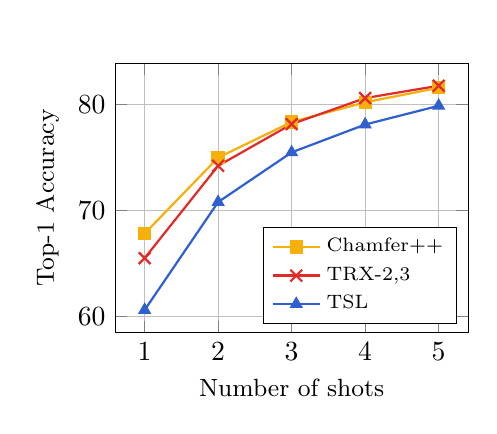
\begin{tikzpicture}
  \begin{axis}[
    width=0.5\linewidth,
    height=5cm, 
    xtick = {0,1,2,3,4,5},
  	legend cell align={left},
	legend pos=south east,
    legend style={font=\scriptsize}, 
    grid=both,
    xlabel={\small Number of shots},
    ylabel={\small Top-1 Accuracy},
    title={\ssvtwo}
  ]
    \addplot [thick, color=C3, mark=square*,  mark size=2] coordinates {(1, 67.83) (2, 75) (3, 78.37) (4, 80.23) (5, 81.60)}; 
	\addlegendentry{Chamfer++} 
	
	\addplot [thick, color=C1,  mark=x,  mark size=3] coordinates {(1, 65.5) (2, 74.23) (3, 78.17) (4, 80.63) (5, 81.8)}; 
	\addlegendentry{TRX-{2,3}} 
	  
    \addplot [thick, color=C2, mark=triangle*,  mark size=2] coordinates {(1, 60.6) (2, 70.8) (3, 75.5) (4, 78.13) (5, 79.9)};  
	\addlegendentry{TSL}
	
  \end{axis}
\end{tikzpicture}

\definecolor{C1}{RGB}{226, 43, 41} % trx
\definecolor{C2}{RGB}{47, 96, 206} % tsl
\definecolor{C3}{RGB}{246, 175, 11} % chamfer

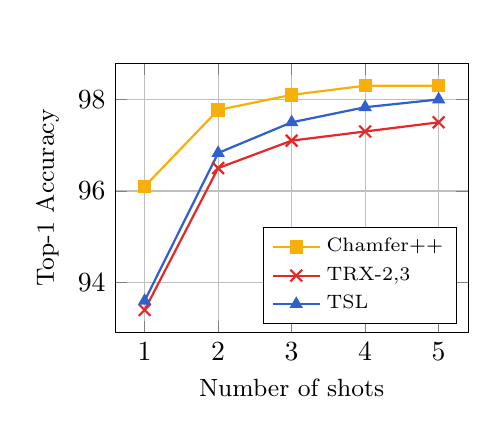
\begin{tikzpicture}
  \begin{axis}[
    width=0.5\linewidth,
    height=5cm, 
    xtick = {0,1,2,3,4,5},
  	legend cell align={left},
	legend pos=south east,
    legend style={font=\scriptsize}, 
    grid=both,
    xlabel={\small Number of shots},
    ylabel={\small Top-1 Accuracy},
    title={\kinetics}
  ]
    \addplot [thick, color=C3, mark=square*,  mark size=2] coordinates {(1, 96.10) (2, 97.77) (3, 98.1) (4, 98.3) (5, 98.30)}; 
	\addlegendentry{Chamfer++} 
	
	\addplot [thick, color=C1,  mark=x,  mark size=3] coordinates {(1, 93.4) (2, 96.5) (3, 97.1) (4, 97.3) (5, 97.5)}; 
	\addlegendentry{TRX-{2,3}}]
    
    \addplot [thick, color=C2, mark=triangle*,  mark size=2] coordinates {(1, 93.6) (2, 96.83) (3, 97.5) (4, 97.83) (5, 98)};  
	\addlegendentry{TSL} 
 
  \end{axis}
\end{tikzpicture}

\end{tabular}
\definecolor{C1}{RGB}{226, 43, 41} % trx
\definecolor{C2}{RGB}{47, 96, 206} % tsl
\definecolor{C3}{RGB}{246, 175, 11} % chamfer

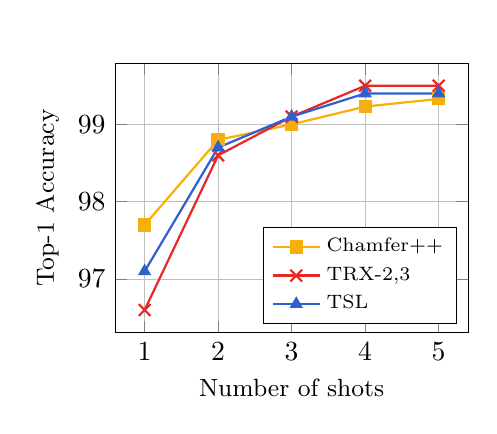
\begin{tikzpicture}
  \begin{axis}[
    width=0.5\linewidth,
    height=5cm, 
    xtick = {0,1,2,3,4,5},
  	legend cell align={left},
	legend pos=south east,
    legend style={font=\scriptsize}, 
    grid=both,
    xlabel={\small Number of shots},
    ylabel={\small Top-1 Accuracy},
    title={\ucf}
  ]
    \addplot [thick, color=C3, mark=square*,  mark size=2] coordinates {(1, 97.7) (2, 98.8) (3, 99) (4, 99.23) (5, 99.33)}; 
	\addlegendentry{Chamfer++}  
	
	\addplot [thick, color=C1,  mark=x,  mark size=3] coordinates {(1, 96.6) (2, 98.6) (3, 99.1) (4, 99.5) (5, 99.5)};   
	\addlegendentry{TRX-{2,3}}]
    
    \addplot [thick, color=C2, mark=triangle*,  mark size=2] coordinates {(1, 97.1)(2, 98.7) (3, 99.1) (4, 99.4) (5, 99.4)};  
	\addlegendentry{TSL}  
	
  \end{axis}
\end{tikzpicture}

\vspace{-0.5ex}
\caption{\textbf{Evolution of the accuracy with the number of examples per class} in the support set for the three datasets.
\label{fig:multi-shots}
}
\end{figure*}


